% !TEX root = ../thesis.tex
%
\chapter{Background and Motivation}%
\label{sec:background}

In this chapter, we are going to introduce the parallelism frameworks \emph{Software Transactional Memory} and \emph{Ohua} as a foundation for the following chapters.
We will briefly present each frameworks' basic concepts as well as advantages and drawbacks to adduce for the following comparison.
To better understand how one can make a well-founded comparison between both concepts, we will also introduce the class of \emph{Irregular Applications} as well as the term \emph{Amorphous Data Parallelism} since both describe important properties encountered in many shared state applications.
We will also briefly discuss the difficulties that arise when reasoning about said application types and motivate, why further research into this topic could prove valuable.

\section{Software Transactional Memory}
\label{sec:background:stm}

With the invention of multi-threaded programming, a need for synchronization primitives arose to allow safe parallelization of data-processing applications.
Usually, locks have been used by developers to guard access to pieces of shared data.

Lock-based programming however, has the fundamental drawback of easily producing deadlocks (i.e., a state where a number of threads may never again progress) when acquiring locks in the wrong order, forcing developers to employ great care when using them.
This results in a lack of composability, as combining several small lock-based modules into a larger program would require the imposition of some sort of ordering on the locks, which frequently leads to problems.
Even when written correctly, lock-based programs tend to quickly become hard to read and maintain due to the many rules that need to be enforced by the programmer herself without any external checks.
Another problem is lock contention.
If a lock is currently taken, all other threads seeking to acquire it have to wait.
This opens up a new set of problems, as frequent waiting leads to prolonged execution times and waiting threads can starve, should the thread fail to release the lock for any reason.
Mitigating contention issues forces developers to consider the trade-off between the overhead introduced by many fine-grained locks, resulting in a higher chance of an accidental deadlock, and high contention.

\begin{figure}[h]
    \begin{subfigure}[h]{\textwidth}
    \begin{minted}{Rust}
        let data = TVar::new(12);   // data is a transaction variable
        thread::spawn(move || {
            atomically(|trans| {    // closure for transaction blocks
                let local = data.read(trans)?;
                data.write(trans, local + 2)
            })});
        thread::spawn(move || {
            atomically(|trans| {
                let local = data.read(trans)?;
                data.write(trans, local * 2)
            })});
    \end{minted}
    \caption{Rust code for both transactions.}%
    \label{fig:background:stmcode}
    \end{subfigure}
    \begin{subfigure}[h]{\textwidth}
    \centering
    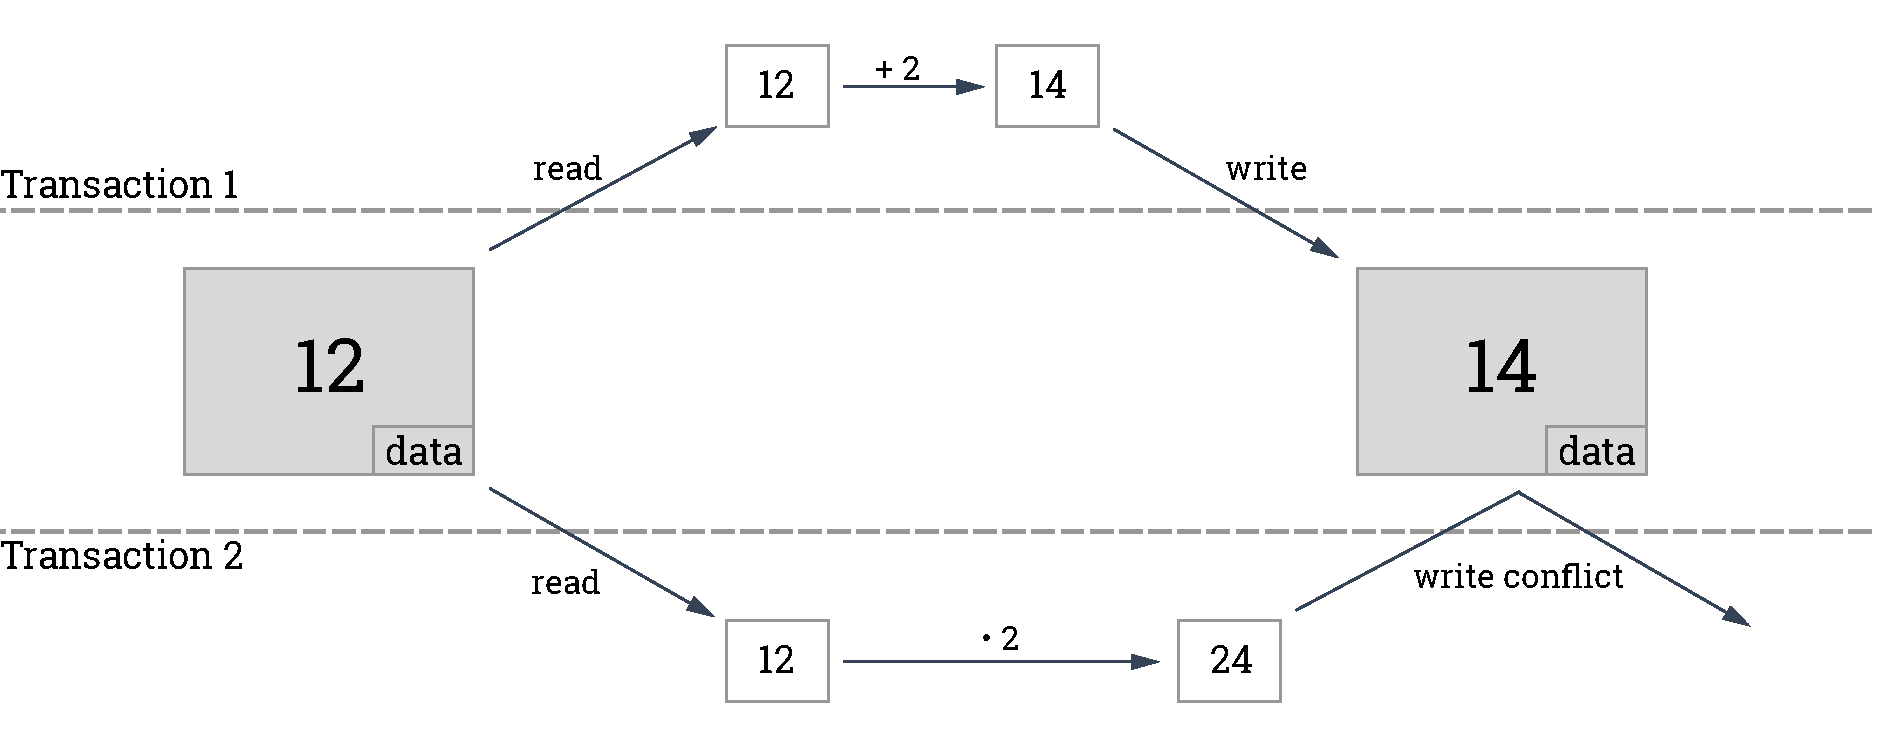
\includegraphics[width=.9\textwidth,keepaspectratio]{gfx/background-stm}
    \caption{Sample execution of two parallel transactions where one transaction has to be rolled back due to a write conflict.}%
    \label{fig:background:stmflow}
    \end{subfigure}
    \caption{Example of two transactions modifying the same shared value in different transactions.}%
    \label{fig:background:stm}
\end{figure}

Hence, Shavit et al.~\cite{shavit1997software} proposed a concept called \emph{Software Transactional Memory}.
This new approach to synchronization aimed to provide lock-free parallelism abstractions that allow multiple threads access to a shared variable without any form of blocking.
Former critical sections are now regarded as \emph{transactions}: They are either executed in their entirety with all their changes taking effect simultaneously or are not executed at all, just like transactions in databases.
STM's operating principle is outlined in Figure~\ref{fig:background:stm} along with a code example in Fig.~\ref{fig:background:stmcode}.
Every read and write operation to or from a piece of shared data is conducted inside a transaction block and gets initially saved to a local transaction log.
When the transaction block comes to an end, the changes made to individual shared data sections are committed.
Therefore, the changes in the log are applied to the original shared values.
In case another transaction managed to commit in the meantime to a value our transaction also touched, the conflict is detected and instead of committing the changes the transaction is aborted and restarted.
This is normally done until the transaction committed successfully.

In our example in Fig.~\ref{fig:background:stm}, the transactions 1 and 2 both read the same value and modify it.
But since the first transaction was able to commit earlier, the second transaction now stands in conflict and has to be aborted and scheduled for re-execution.

As the example already shows, a fundamental benefit of the (Software) Transactional Memory model is its serializability~\cite{swalens2016transactional}:
All transactions seem to execute serially, since the steps of one transaction never appear to be interleaved with the steps of another transaction.
Therefore, the results of an execution must be equal to the result of a serial execution.
This has been formalized by Swalens et al.~\cite{swalens2016transactional} in their proposed operational semantics for a language with transactions.

Overall, STM takes an optimistic approach to parallelism, because it simply executes numerous computations without any heuristics or reasoning in parallel, hoping for as few conflicts as possible.
The result of this is an underlying non-determinism that ensues everytime transactions are employed in a multi-threaded environment.
Problems in this strategy become apparent when applied to high-contention scenarios.
Since STM may work in parallel over the same data structure or memory region, high contention always leads to a significantly increased number of retries for individual executions, which in turn leads to drastically reduced performance.
Further shortcomings of this concept have been discussed in detail by Caşcaval et al.~\cite{cascaval2008software}:
On the one hand, exception handling becomes impossible to do inside of a transaction without breaking its semantics.
On the other hand, I/O operations cannot be transactionalized, as well as anything else that produces side effects outside of the transactions' scope as these effects may not be rolled back on error.
Additionally, they reported large overheads of STM applications for smaller worksets as well as no debuggability, since the non-determinism makes a specific situation nearly irreproducible.


\section{Ohua}
\label{sec:background:ohua}

As we have seen before, most frameworks for parallel programming offer developers certain abstractions or data structures such as threads, locks or transactions for them to use when developing parallel programs.
This however, forces programmers to think within the boundaries of their chosen tools and produces code that is tailored to a specific framework and therefore hard to migrate.

A completely different approach has been taken by Ertel et al.~\cite{ertel2019dis} with the proposition of \emph{Ohua}, which is a framework that allows the development of implicitly parallel programs.
It consists of three main components, as outlined in Fig.~\ref{fig:background:ohua}:
\emph{Algorithms}, which are used to describe the program part that shall be parallelized, a \emph{compiler} that interprets the algorithm and produces a parallelized version of it and a \emph{runtime} that will execute the parallel code.

\begin{figure}[h]
    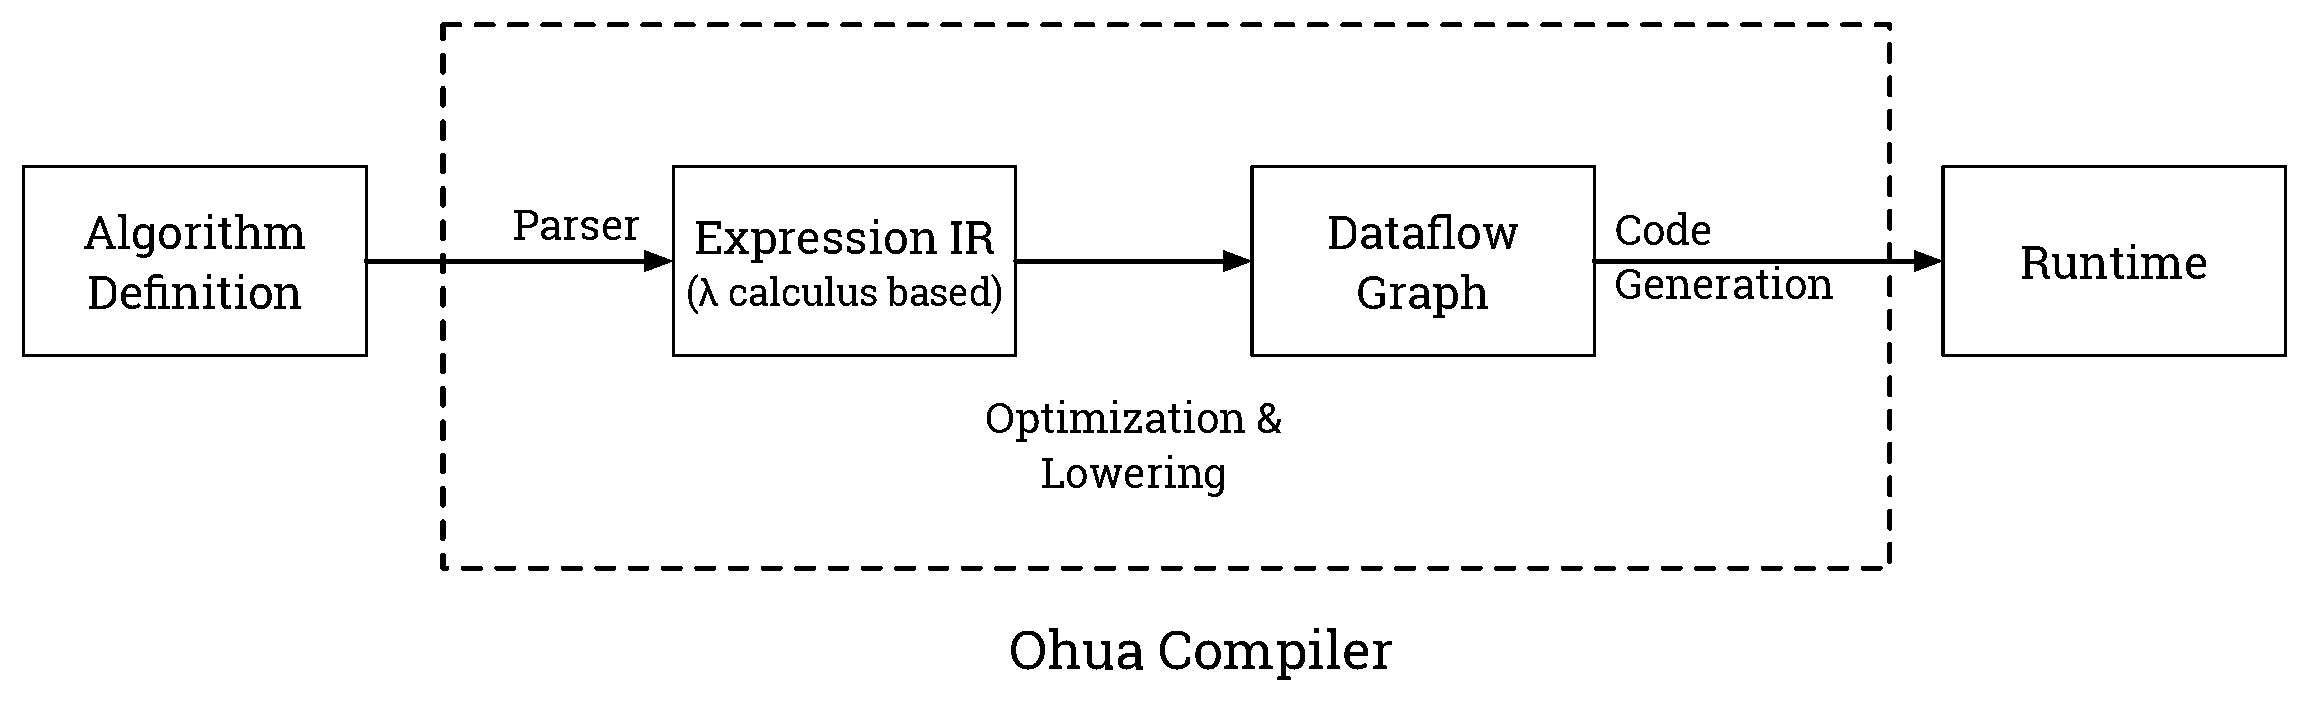
\includegraphics[width=\textwidth,keepaspectratio]{gfx/background-ohua}
    \caption{Overview of the Ohua compiler and its components}%
    \label{fig:background:ohua}
\end{figure}

An Ohua algorithm is what might come closest to the abstractions and tools used by other paradigms.
It describes the part of a program that should be turned into a parallelized runtime.
In early versions~\cite{ertel2015ohua} these algorithms were written in separate files using a high-level language that closely resembled Lisp and OCaml.
Over time, a Rust-like syntax~\cite{adam2019master} had also been added to allow for more imperative algorithm definitions.
By now, algorithms are not separately defined anymore and instead are functions that are written in a host language which is supported by Ohua, such as Rust and Go.
Ohua comes with a standalone compiler called \rust{ohuac}, which proceeds to parse the algorithm into an Expression IR, optimizes it and eventually transforms it into an optimized dataflow graph.
These optimizations stem from a number of transformations that are applied to uncover more parallelism opportunities.
A host language specific backend will then generate the runtime code based on the DFG.
This runtime executes as regular part of the program it is embedded in when the algorithm is called.
As such, it may import and use any function from the host code, allowing the developer seamless integration of her existing code into the new parallel algorithm.

Ohua derives parallelism from executing independent nodes of the dataflow graph in parallel (task-level parallelism) and running multiple invocations of dependent nodes in a pipeline-parallel fashion.
In order to rule out most of the common pitfalls in parallel programming, the use of shared state is forbidden in Ohua.
Instead, data must be transferred explicitly by using arguments and function return values.
This also rules out mutable global values which often represent state in programs.
To still allow the convenient declaration of stateful algorithms, Ohua uses the concept of so-called \emph{stateful functions}~\cite{ertel2019stclang}.
A stateful function is a host function that is associated with local state values which it is allowed to modify.
Ohua encapsulates this operation and the associated state to ensure it is not leaked or used in a shared fashion.

\begin{figure}[h]
    \begin{subfigure}[h]{.5\textwidth}
        \begin{minted}{Rust}
            let words = vec!["a", "test"];
            let buffer = Buffer::new();
            let _ = for w in words {
                buffer.append(w);
            };
            buffer.get_message();
        \end{minted}
        \caption{Algorithm declaration in Rust}
        \label{fig:backend:smap:algo}
    \end{subfigure}
    \begin{subfigure}[h]{.5\textwidth}
        \missingfigure{Add DFG}
        \caption{The algorithm's dataflow graph. Dependencies in the control flow are dotted.}
        \label{fig:backend:smap:dfg}
    \end{subfigure}
    \caption{Example of an Ohua algorithm using the \rust{smap} primitive.}%
    \label{fig:background:smap}
\end{figure}

Ertel et al.\ additionally proposed \rust{smap}, a stateful map primitive that applies an algorithm to a sequence of items~\cite{ertel2019stclang} and is based on the insight, that loop operations modifying shared state can be considered as fold operations on the state.
An example algorithm in Rust that outlines this is shown in Fig.~\ref{fig:background:smap}.
Functions highlighted in red are builtin functions of the Ohua runtime, all other nodes are host functions provided by the developer.
In our example, the \rust{smap} primitive is represented by the for loop and its use of the \rust{buffer} variable in the body.
The loop body is applied to a sequence of items, just as it would happen in a normal \rust{map} statement.
But additionally, \rust{smap} ensures that changes made to the encapsulated state persist, as they would in a normal \rust{for} loop.
This allows the use of pipeline parallelism for longer loop bodies and -- if no state is used in the loop at all -- the use of data parallelism.
So in Fig.~\ref{fig:background:smap}, the newly initialized buffer is bound to the \rust{append} function, which is called like a method on the state repeatedly for the individual loop iterations.
Any results which would be produced by this loop, are then collected and upon completion of the loop passed on to the next node in the dataflow graph.
In the small code snippet provided, an iteration simply produces a \rust{()} literal\footnote{The \rust{()} type is called Unit literal in Rust. It is the result of a computation that returns nothing and can be compared to the \rust{void} type in C.} and hence the loop result itself is discarded.
What remains, is the side effect of state alteration that occured during the loop processing.
After the loop completes, the next function is executed.
To avoid \rust{get_message} being called too early, a control flow dependency is added to the (otherwise useless) \rust{collect} function.

The result of Ohua's programming model is \emph{deterministic parallelism}, as opposed to Software Transactional Memory which aims to improve execution times by scheduling possibly conflicting operations for parallel execution, completely forfeiting any determinism in the process.
Another advantage is the way in which Ohua is integrated into existing code bases.
In its current version, algorithms are defined as normal functions within the code, allowing developers to first test their implementations without any parallelism before compiling them with Ohua.
This offers the advantage of producing framework agnostic code which can be easily reused in other applications as well.

Challenging however, is the ban the framework places on the use of shared state.
Many applications encountered in the real world rely on the use of pointers and shared, global state.
Since Ohua currently only fosters the use of local state with its stateful functions primitives, it is unclear whether it is possible to apply these concepts to shared state programs, which the Software Transactional Memory framework caters towards by design.


\section{Irregular Applications}
\label{sec:background:irregular}

Providing a comprehensive comparison between STM and Ohua requires a selection of representative shared state applications to test both systems on.
But to make such a selection, one first has to understand, which features describe such an application and how these properties may influence the parallel behavior as well as the viability of certain parallelism frameworks.
In the past, most of the research conducted in the field of performance improvements for parallel programs has concerned itself with what is called regular applications.
These are applications, whose degree of exploitable parallelism is simply determined by the program structure and the size of the input set.
As both of there properties are known or can be inferred at compile time, any optimization potential is easy to uncover and exploit for compilers.

When looking at \emph{irregular applications} on the other hand, the situation is completely different.
The term describes applications, whose structure resolves around the manipulation of large, pointer-based data structures like graphs and trees.
Due to this structural peculiarity, compiler analyses struggle to uncover any meaningful insights into the algorithm that would allow to exploit any parallelism hidden in it.

\begin{figure}[b]
    \centering
    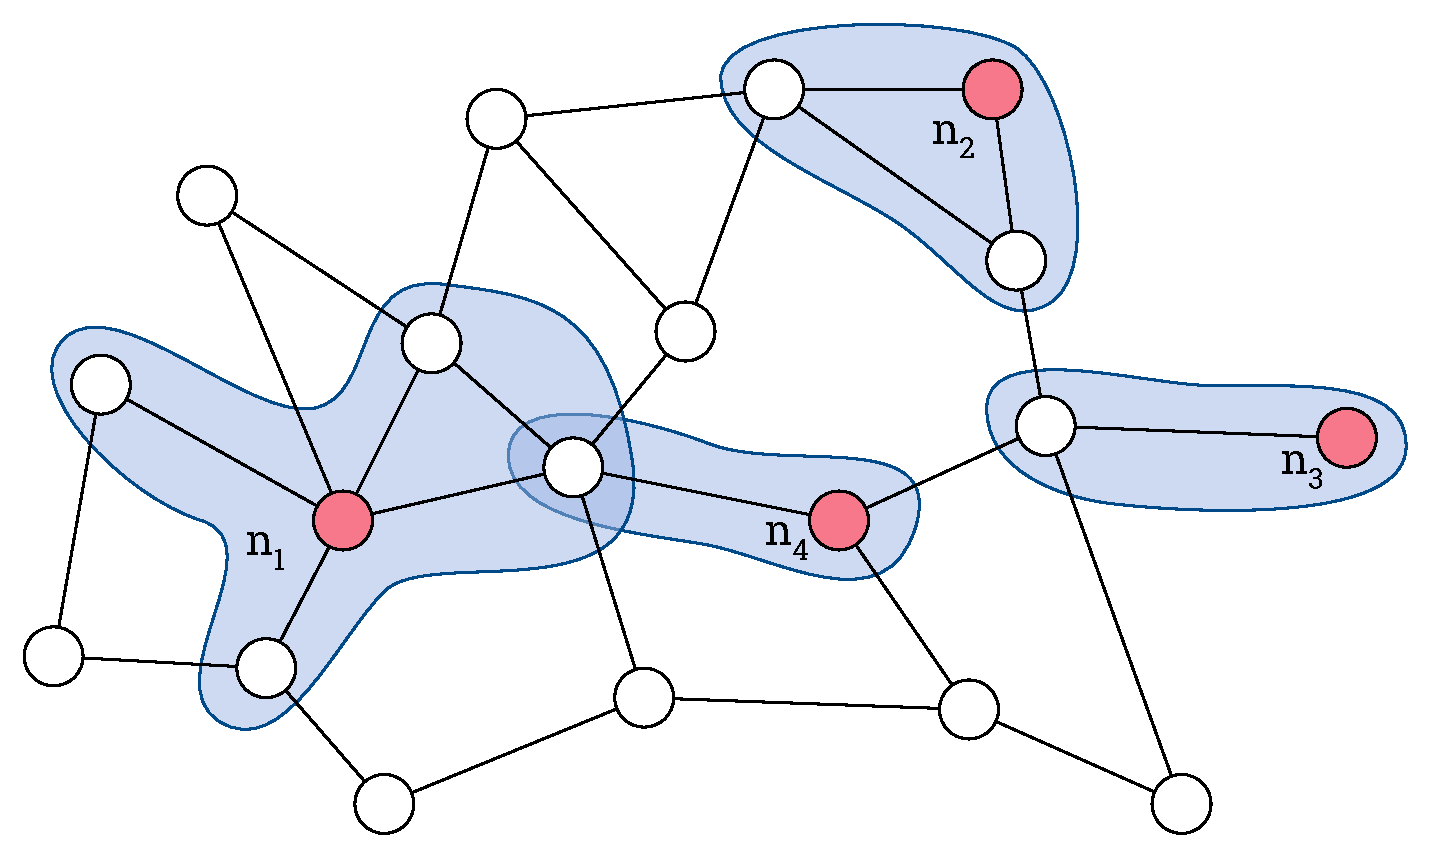
\includegraphics[width=.7\textwidth,keepaspectratio]{gfx/background-irregular}
    \caption{Graph representation of an irregular application with active elements and their neighborhoods. Adapted from Kulkarni et al.~\cite{kulkarni2009much}}%
    \label{fig:background:irregular}
\end{figure}

To better outline this, Kulkarni et al.~\cite{kulkarni2009much} developed an abstract representation for irregular programs using a set of nodes and edges, as shown in Fig.~\ref{fig:background:irregular}.
The nodes and edges represent the input data and their relationships.
During the execution of an irregular algorithm, the program may perform computations on a (sub-)set of active nodes or edges, the work items.
In Figure~\ref{fig:background:irregular}, these are highlighted in red.
Performing said executions may involve reading from or writing to other nodes or edges in the graph, which form an active elements' neighborhood, shaded in blue.
Which elements of the graph make up the neighborhood of an active element is not known beforehand and may encompass all direct neighbors in the graph (as seen for nodes $n_2$ and $n_3$), maybe only a single neighboring element (as seen for node $n_4$) or transitively the neighboring elements of its direct neighbors.

Usually, work items are not ordered and may be processed in any order.
But processing one element may generate an arbitrary number of new active elements or remove others from the pool, depending on the algorithm.
Also, some active elements may not be processed simultaneously due to overlapping neighborhoods, as the changes made by processing both items may conflict with each other.

Since all these relationships and interdependencies are not known beforehand but rather depend on the input data, this information cannot be uncovered and used by compile time analyses.
Yet, most shared state applications are irregular applications by design, making this a large and interesting field of research.
Because static parallelization as well as lock-based approaches fail to uncover any viable parallelism opportunities in these programs, Kulkarni et al.~\cite{kulkarni2007optimistic} argue, that optimistic strategies such as \emph{Software Transactional Memory} need to be used to tackle this class of problems.
This is because, as we have shown, the heavy use of pointers in the program hinders efficient analyses but as conflicts due to parallelization may be rare (depending on the input data) the optimistic trial-and-abort semantics of STM allow for a simple and efficient parallelization in most cases.
As of now, it is unclear whether Ohua could also be used to parallelize irregular applications, offering an alternative besides STM for this type of applications where most other frameworks fail.
Since its approach relies heavily on compile-time analyses and optimizations, it may prove challenging to try to uncover good parallelism opportunities here.


\subsection{Amorphous Data Parallelism}
\label{sec:background:irregular:adp}

Pingali et al.~\cite{pingali2009amorphous} argue, that most irregular applications additionally exhibit a behavior referred to as \emph{amorphous data parallelism}:

Given a set of active nodes and an ordering on them, amorphous data parallelism is the parallelism that arises from simultaneously processing active nodes and is subject to neighborhood and ordering constraints.
It is a generalization of standard data parallelism in which
\begin{enumerate}
    \item concurrent operations may conflict with each other
    \item activities can be created dynamically
    \item activities may modify the underlying data structure
\end{enumerate}
These characteristics have already been briefly discussed in connection with Fig.~\ref{fig:background:irregular}.

While irregular applications are hard to reason about due to their pointer usage, they are still a very interesting research topic, made more difficult by amorphous data parallelism.
But as we will show in Chapter~\ref{sec:experiments}, applications of this type are common and widespread in different aspects of real world applications using shared state.




% - present both Ohua and STM
%   - explain paradigms in detail (most people here don't know what stm is and how it works!)
%   - detail benefits and shortcomings of both
%   - Ohua: talk about the compiler, its stages and where optimizations hook in as this will be required information later on.
%   - STM: Detail that non-determinism is part of the execution model -> speculative parallelism
%       - make sure to thoroughly explain the concept of a transaction
%   - Ohua: detail determinism of the model if appropriate, but remember that this will also be discussed later on
% - explain Irregular Applications: They are different from the parallelizability problems we usually face as the input dictates the parallelism at runtime and the computing times!
%   - use: \label{sec:background:irregular}
